Fadenpendel & 
\begin{minipage}{11cm}
	$\vec{F}_G = \vec{F}_{rad} + \vec{F}_{tan}$\newline 
	nur $\vec{F}_{tan}$ berücksichtigen, da $\vec{F}_{rad}$ von 'Fadenkraft' kompensiert wird
	$\vec{F}_{tan} = -|\vec{F}_g|\cdot \sin(\varphi) = -mg \sin(\varphi)$\qquad 
	$ a(t) = \dot v(t) = l\dot \omega(t) = l\ddot \varphi(t) $
	$\vec{F}_{tan} = m \cdot a_{tan} = m\cdot l\ddot \varphi(t) = -mg\sin(\varphi) \implies$ \newline 
	$l\cdot \ddot \varphi(t) + g\sin(\varphi) = 0 \qquad \text{Taylor } \sin(\varphi) \approx \varphi$\newline  
	$l\cdot \ddot \varphi + g\cdot \varphi =0 \qquad \text{DGL lösen}$\newline 
	Ansatz: $\varphi(t) = e^{\lambda t} \qquad l\lambda^2 e^{\lambda t} + g e^{\lambda t} = 0$\newline
	$l\lambda^2 + g = 0 \qquad \lambda = \pm j\sqrt{\frac{g}{l}} \qquad \varphi(t) = A\sin\sqrt{\frac{g}{l}} + B\cos\sqrt{\frac{g}{l}}$\newline
	$\hat\varphi = \sqrt{B^2+ A^2}\qquad \varphi_0 = \frac{B}{A}\qquad \boxed{\varphi(t) = \hat \varphi\cdot \sin\left( \sqrt{\frac{g}{l}} + \varphi_0 \right)}$ 
\end{minipage}\begin{minipage}{3cm}
	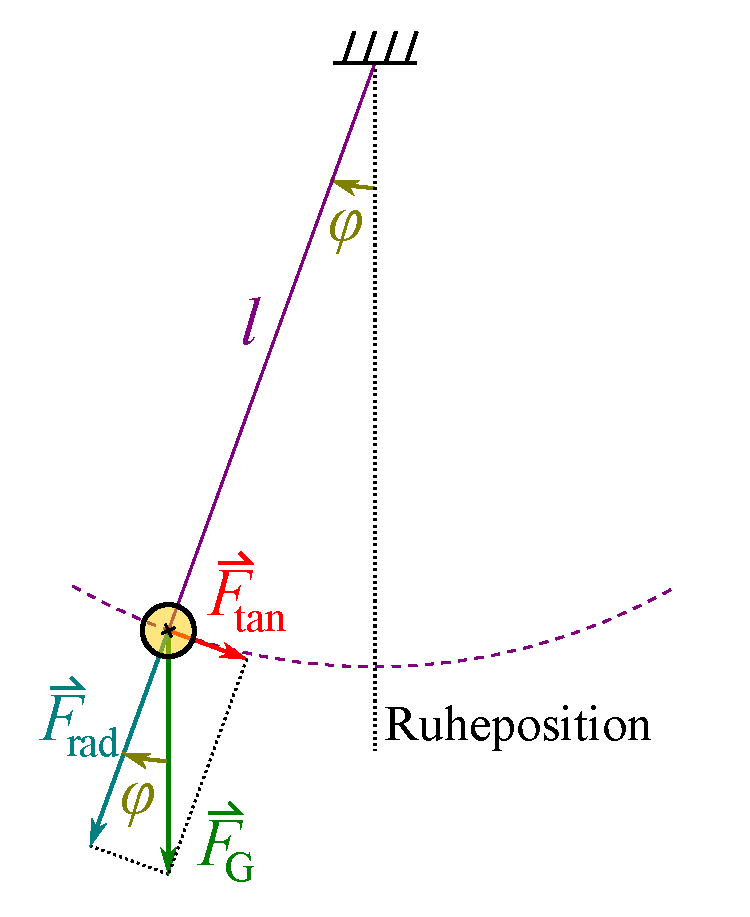
\includegraphics[width = 3cm]{images/fadenpendel}
\end{minipage}





\\	